\chapter{Plataforma de desarrollo}
\label{cap:capitulo4}

\begin{flushright}
\begin{minipage}[]{10cm}
\emph{Las herramientas adecuadas en las manos adecuadas pueden cambiar el mundo}\\
\end{minipage}\\
Steve Jobs\\
\end{flushright}

\vspace{1cm}
Tras haber establecido los objetivos que se pretenden alcanzar en este trabajo de fin de grado, se procede a describir
las herramientas \textit{software} y \textit{hardware} utilizadas para lograrlos. 

\section{Software}
\label{sec:software}
Llamamos \textit{software} al conjunto de programas, instrucciones y datos que dotan de lógica al sistema.
\subsection{Python}
\label{subsec:pyhton}
Python es un lenguaje de programación, es decir, una serie de reglas gramaticales bien definidas que le proporciona a una persona, en este 
caso el programador, la capacidad de programar una serie de instrucciones o secuencias de órdenes con el fin de crear un comportamiento 
lógico determinado. 

Se trata de un lenguaje de alto nivel interpretado. Cuando se dice que un lenguaje es de alto nivel, se hace referencia a su nivel de 
abstracción y facilidad de uso en comparación con los lenguajes de bajo nivel, es decir, aquellos que te permiten mayor control sobre los 
componentes físicos del sistema. Decimos que es un lenguaje interpretado debido a que no es necesario convertir el texto escrito por el humano en 
instrucciones entendibles por un procesador previamente a su ejecución. Esto agiliza el proceso de desarrollo ya que la conversión de código humano a 
código máquina (compilación) suele demorar un tiempo. Por el contrario, la ejecución de un programa en lenguaje compilado es más rápida.  

Una de las características más destacadas de Python es su amplia librería (conjunto de código destinado a un objetivo concreto) estándar, que proporciona 
variedad de módulos y funciones para realizar multitud de tareas. Como cualquier otro lenguaje de programación, cuenta con una gran cantidad de librerías de terceros que 
amplían sus capacidades, como SciPy en la ciencia de datos, Django en el desarrollo web, Numpy para operar con matrices, TensorFlow el aprendizaje automático, entre otros.

\subsection{Grbl}
\label{subsec:grbl}
Grbl\footnote{\url{https://github.com/gnea/grbl}} es un firmware de código abierto usado para controlar máquinas llamadas \acs{CNC}. Este firmware se ejecuta en 
un microcontrolador, que se encuentra dentro de la controladora de la máquina \acs{CNC}, en nuestro caso, la placa base del robot. \\
Básicamente, convierte las instrucciones de código G, que posteriormente hablaremos de él, en señales eléctricas que se envían a los motores de la máquina. Además, 
comprueba los diferentes sensores de la máquina, como pueden ser los finales de carrera, para establecer los límites físicos de cada movimiento. \\
Grbl es flexible por lo que podemos cambiar la configuración para adaptarla a un caso de uso concreto. De hecho, aunque solo soporta movimientos lineales,
en este trabajo se abordará la configuración necesaria para para poder usar las articulaciones rotativas del nuestro robot.

\subsection{ROS 2}
\label{subsec:ros2}
ROS, por sus siglas en inglés, significa \textit{Robot Operating System}. Se trata de una plataforma de código abierto utilizada 
para desarrollar y controlar sistemas robóticos.
El objetivo principal de ROS es facilitar el desarrollo de sistemas robóticos al proporcionar una infraestructura que permite que
los desarrolladores pueden centrarse en la lógica y el comportamiento específico de los robots, sin tener que preocuparse por la 
infraestructura de comunicación y control. 
Además, proporciona una colección de bibliotecas, herramientas y convenios que permiten a los programadores crear software para robots. 
También proporciona herramientas para la visualización de datos, simulación de robots, depuración y pruebas. Además, 
cuenta con una comunidad activa de usuarios y desarrolladores que contribuyen con paquetes adicionales y comparten su 
conocimiento.

Está diseñado para ser modular, lo que permite la creación de sistemas complejos mediante la reutilización de otros componentes existentes.

Una de las características distintivas de ROS es su arquitectura basada en nodos. Los nodos son procesos independientes 
que se comunican entre sí mediante mensajes. Cada nodo puede realizar tareas específicas, en función de la lógica atribuída por el programador.

En este trabajo se utiliza ROS 2, la versión sucesora de ROS. Esta versión incorpora gran variedad de mejoras respecto a su anterior versión. En esta versión 
los nodos no dependen de un nodo \textit{Master} para comunicarse ya que las comunicaciones están distribuidas mediante el uso de \ac{DDS}. Esto 
incrementa la robusted del sistema y reduce significativamente los tiempos de latencia. \\
La distribución de utilizada en este trabajo es \textit{ROS 2 Humble}. Se trata de la última versión de ROS estable disponible para Ubuntu 22.04 LTS.
\begin{figure} [h!]
  \begin{center}
    
\includegraphics[width=4cm]{figs/ros2logo.jpeg}
  \end{center}
  \caption{Logotipo de ROS 2 Humble}
  \label{fig:ros2logo}
\end{figure}\ 

\subsection{MoveIt!}
\label{subsec:moveit}

\section{Hardware}
\label{sec:hardware}
Cuando hablamos de \textit{hardware}, nos referimos a todos los componentes físicos de utilizados en el dispositivo electrónico, en este caso, un robot. Estos 
componentes son tangibles, es decir, se pueden tocar y ver.
\subsection{Código G}
\label{sec:gcode}
Se trata 

\section{MKS DLC32}
\label{subsec:mksdlc32}
Se trata de una placa destinada al mundo de las máquinas de grabado láser. Ha sido creada por \textit{MakerBase} y es considerada 
\textit{Open Hardware} por lo que toda la información de la placa puede encontrarse en su repositorio de Github\footnote{\url{https://github.com/makerbase-mks/MKS-DLC32}}.
Es fácilmente adquirible por \textit{Aliexpress} por un precio que ronda los 16\euro. Está basada en el microcontrolador de 32 bits: ESP32. 
Se trata de un dispositivo muy asentado en la comunidad \textit{maker} debido a su bajo coste e integración en el 
ecosistema Arduino. De hecho, gracias a su conectividad wifi y bluetooth ha ganado terreno a los microcontroladores Atmega que incorporan los propios Arduinos.\\
Esta placa es ideal para este proyecto debido a que cuenta con la posibilidad de controlar 
hasta 3 motores y es completamente compatible con \nameref{subsec:grbl}. Además dispone de una salida de potencia regulable controlable mediante \nameref{subsec:grbl} que nos 
permite alimentar dispositivos. Estos podrían ser: electroimán (tipo de imán que es activado mediante electricidad), motor \ac{CC} entre otros. Además se puede aprovechar las salidas \ac{PWM} para conectar un grabador láser o un servo. 
El rango de funcionamiento es de 12 a 24 voltios por lo que es adecuado para ser alimentado mediante baterías y con cargadores de ordenador. 
\begin{figure} [h!]
    \begin{center}
      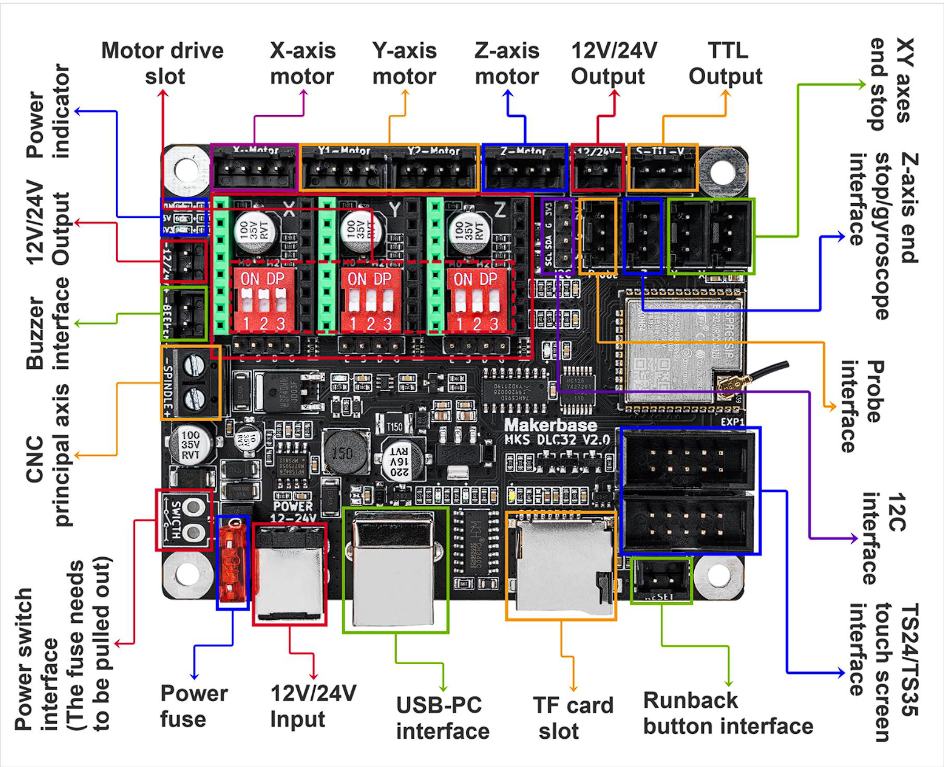
\includegraphics[width=8cm]{figs/MKS.png}
    \end{center}
    \caption{Placa base MakerBase DLC32}
    \label{fig:robSoldering}
  \end{figure}\ 

\section{Motores Nema 17}
\label{subsec:motores}
Un motor paso a paso es un tipo de motor que se mueve en pequeños pasos o incrementos discretos en lugar de girar continuamente. Estos pasos 
son controlados por señales eléctricas que hacen girar al motor una cantidad específica de grados cada vez que se envía una señal. Debido a que se tiene 
control sobre su avance son una excelente opción si se quiere tener un motor que sea capaz de posicionarse en un ángulo concreto con exactitud. A pesar
de su gran precisión, los motores paso a paso convencionales no tienen el conocimiento absoluto de su posición, por lo que todos los movimientos son 
relativos. Esto hace que se requiera de un \textit{homing} (proceso en el cual la máquina CNC lleva las partes móviles a una 
posición conocida) en el arranque de la máquina para conocer su estado antes de operar.
Para este trabajo, se han usado 3 motores Nema 17 de 60 milímetros de largo debido a las necesidades calculadas más adelante. Son motores bipolares de 
2.1 amperios y una resistencia de 1,6 ohmios con un torque máximo de 0.65 newton-metro.
\begin{figure} [h!]
    \begin{center}
      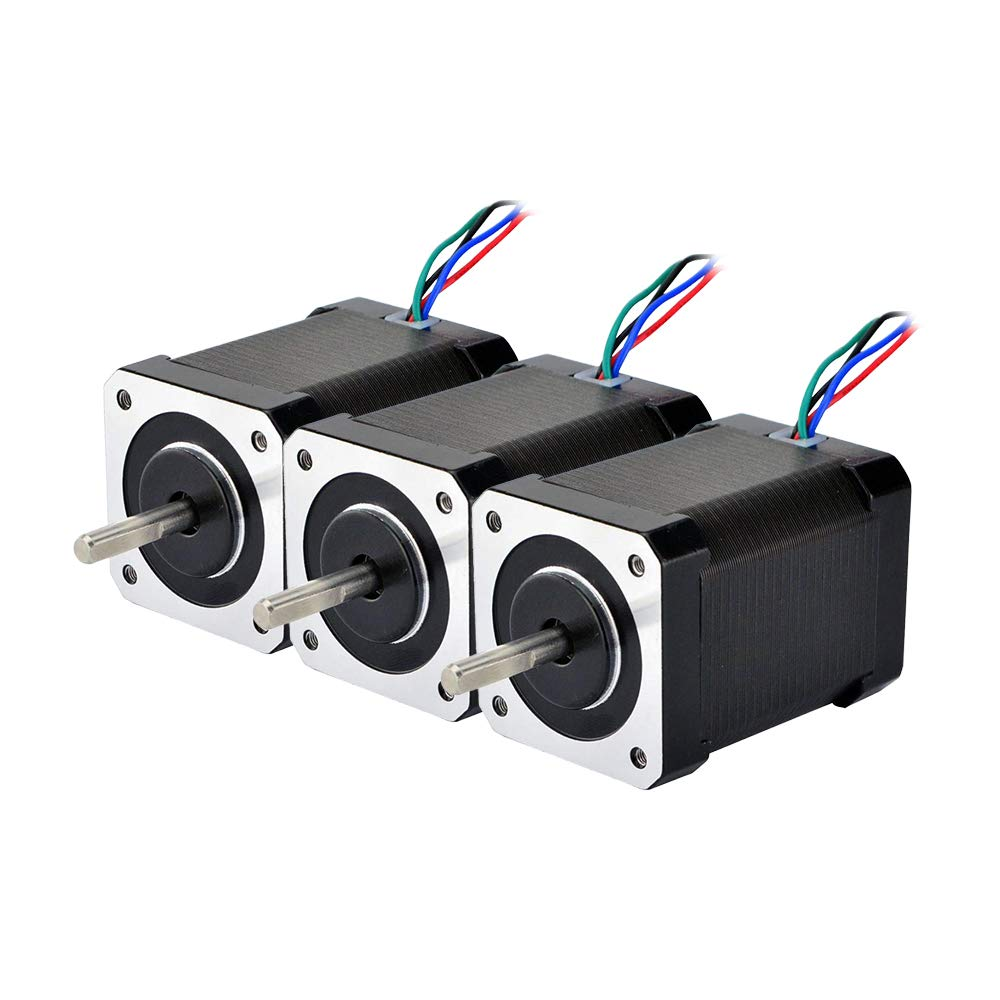
\includegraphics[width=8cm]{figs/nema17.jpg}
    \end{center}
    \caption{Motores Nema 17 de 2.1A}
    \label{fig:robSoldering}
  \end{figure}\ 

\section{Controlador TMC2209}
\label{subsec:controladorPAP}
Un controlador paso a paso es el módulo hardware capaz de trasformar las señales lógicas que le envía el controlador en una serie de pulsos de
potencia que excitarán las bobinas del motor en un cierto orden para lograr el movimiento. 
Existen motores bipolares, unipolares e híbridos. La diferencia entre ellos radica en la disposición de las bobinas de su interior. Los más usados 
en impresoras 3D y CNC son los bipolares. Son reconocibles debido a que tienen 4 cables.
En este tipo de placas base se pueden instalar distintos modelos de controladores. Cada uno de ellos tiene unas prestaciones diferentes y por tanto 
un precio distinto. Unos ofrecen mayor capacidad de corriente (para controlar motores más grandes), pulsos más suaves que reducen el 
ruido sonoro y las vibraciones, medición en tiempo real de la corriente consumida para conocer el final de una articulación, entre otras tecnologías.  
\begin{figure} [h!]
    \begin{center}
      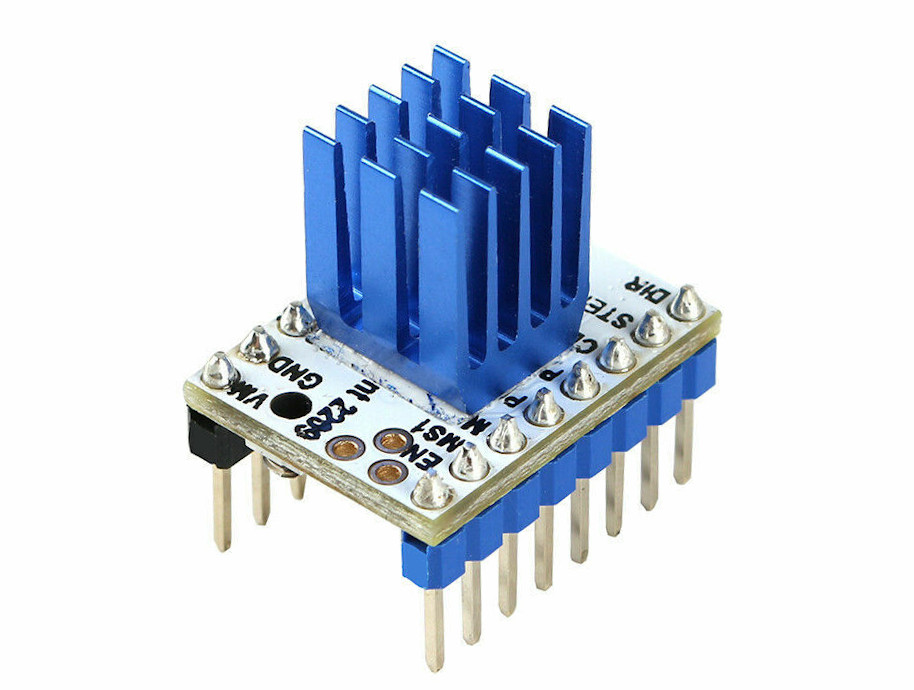
\includegraphics[width=6cm]{figs/TMC2209.jpg}
    \end{center}
    \caption{Controlador TMC2209}
    \label{fig:robSoldering}
  \end{figure}\ 

\section{Fuente de alimentación genérica}
\label{subsec:fuente_alimentacion}
Para alimentar el brazo se va a utilizar una fuente de alimentación genérica de 24 voltios y 6 amperios. Este tipo de fuentes pueden ser 
fácilmente adquiribles por internet por un precio aproximado de 15 \euro. A pesar de esto, puede ser usada cualquier tipo de fuente capaz de 
entregar más de 20 vatios en el rango de voltaje 12-24v. Más adelante se aborda el uso de cargadores de ordenadores portátiles para alimentar el 
brazo.

\begin{figure} [h!]
  \centering    
  \subfigure[Fuente de alimentación 24v 5A]{\label{fig:pw24}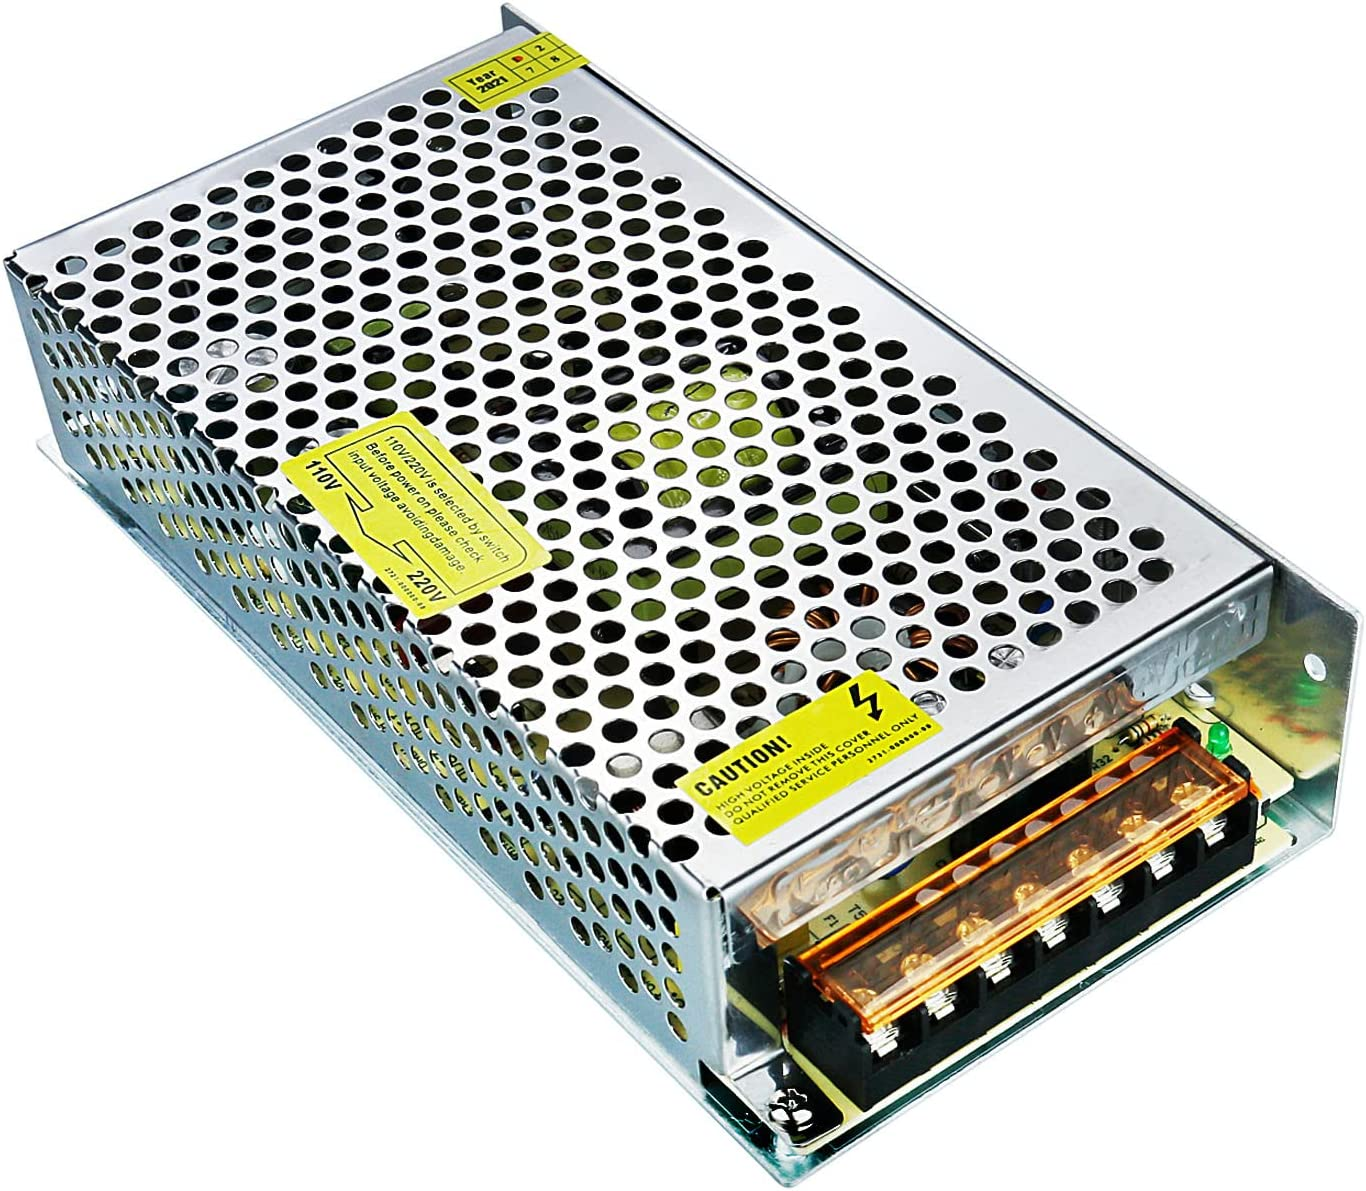
\includegraphics[width=0.4\linewidth ]{figs/pw24v.jpg}}
  \hspace{3cm}
  \subfigure[Cargador de portátil genérico]{\label{fig:pw19}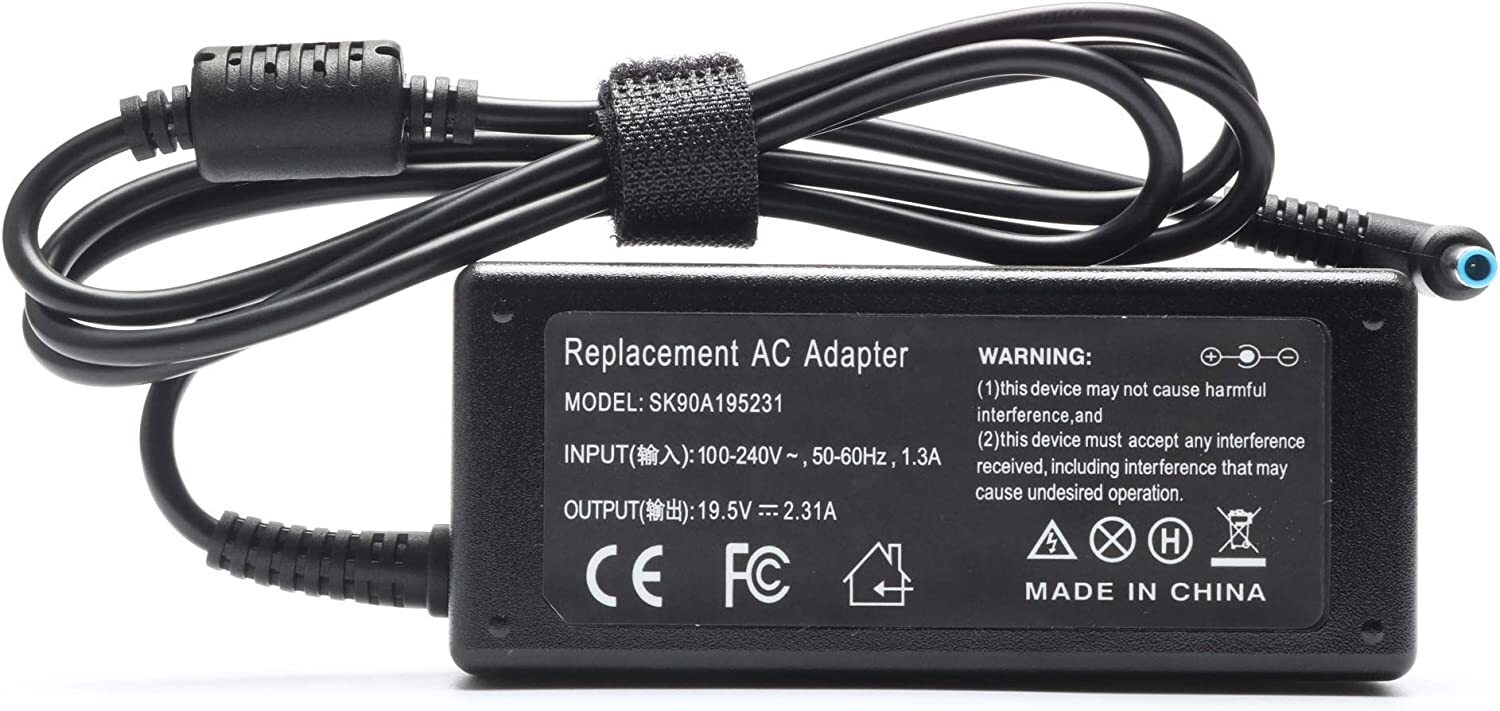
\includegraphics[width=0.4\linewidth]{figs/pw19v.jpg}}
  \caption{Métodos usados para alimentar el robot}
\end{figure}


